\documentclass[]{article}
\usepackage{lmodern}
\usepackage{amssymb,amsmath}
\usepackage{ifxetex,ifluatex}
\usepackage{fixltx2e} % provides \textsubscript
\ifnum 0\ifxetex 1\fi\ifluatex 1\fi=0 % if pdftex
  \usepackage[T1]{fontenc}
  \usepackage[utf8]{inputenc}
\else % if luatex or xelatex
  \ifxetex
    \usepackage{mathspec}
  \else
    \usepackage{fontspec}
  \fi
  \defaultfontfeatures{Ligatures=TeX,Scale=MatchLowercase}
\fi
% use upquote if available, for straight quotes in verbatim environments
\IfFileExists{upquote.sty}{\usepackage{upquote}}{}
% use microtype if available
\IfFileExists{microtype.sty}{%
\usepackage{microtype}
\UseMicrotypeSet[protrusion]{basicmath} % disable protrusion for tt fonts
}{}
\usepackage[margin=1in]{geometry}
\usepackage{hyperref}
\hypersetup{unicode=true,
            pdftitle={hw2},
            pdfauthor={Pablo,Román,Sofía},
            pdfborder={0 0 0},
            breaklinks=true}
\urlstyle{same}  % don't use monospace font for urls
\usepackage{color}
\usepackage{fancyvrb}
\newcommand{\VerbBar}{|}
\newcommand{\VERB}{\Verb[commandchars=\\\{\}]}
\DefineVerbatimEnvironment{Highlighting}{Verbatim}{commandchars=\\\{\}}
% Add ',fontsize=\small' for more characters per line
\usepackage{framed}
\definecolor{shadecolor}{RGB}{248,248,248}
\newenvironment{Shaded}{\begin{snugshade}}{\end{snugshade}}
\newcommand{\AlertTok}[1]{\textcolor[rgb]{0.94,0.16,0.16}{#1}}
\newcommand{\AnnotationTok}[1]{\textcolor[rgb]{0.56,0.35,0.01}{\textbf{\textit{#1}}}}
\newcommand{\AttributeTok}[1]{\textcolor[rgb]{0.77,0.63,0.00}{#1}}
\newcommand{\BaseNTok}[1]{\textcolor[rgb]{0.00,0.00,0.81}{#1}}
\newcommand{\BuiltInTok}[1]{#1}
\newcommand{\CharTok}[1]{\textcolor[rgb]{0.31,0.60,0.02}{#1}}
\newcommand{\CommentTok}[1]{\textcolor[rgb]{0.56,0.35,0.01}{\textit{#1}}}
\newcommand{\CommentVarTok}[1]{\textcolor[rgb]{0.56,0.35,0.01}{\textbf{\textit{#1}}}}
\newcommand{\ConstantTok}[1]{\textcolor[rgb]{0.00,0.00,0.00}{#1}}
\newcommand{\ControlFlowTok}[1]{\textcolor[rgb]{0.13,0.29,0.53}{\textbf{#1}}}
\newcommand{\DataTypeTok}[1]{\textcolor[rgb]{0.13,0.29,0.53}{#1}}
\newcommand{\DecValTok}[1]{\textcolor[rgb]{0.00,0.00,0.81}{#1}}
\newcommand{\DocumentationTok}[1]{\textcolor[rgb]{0.56,0.35,0.01}{\textbf{\textit{#1}}}}
\newcommand{\ErrorTok}[1]{\textcolor[rgb]{0.64,0.00,0.00}{\textbf{#1}}}
\newcommand{\ExtensionTok}[1]{#1}
\newcommand{\FloatTok}[1]{\textcolor[rgb]{0.00,0.00,0.81}{#1}}
\newcommand{\FunctionTok}[1]{\textcolor[rgb]{0.00,0.00,0.00}{#1}}
\newcommand{\ImportTok}[1]{#1}
\newcommand{\InformationTok}[1]{\textcolor[rgb]{0.56,0.35,0.01}{\textbf{\textit{#1}}}}
\newcommand{\KeywordTok}[1]{\textcolor[rgb]{0.13,0.29,0.53}{\textbf{#1}}}
\newcommand{\NormalTok}[1]{#1}
\newcommand{\OperatorTok}[1]{\textcolor[rgb]{0.81,0.36,0.00}{\textbf{#1}}}
\newcommand{\OtherTok}[1]{\textcolor[rgb]{0.56,0.35,0.01}{#1}}
\newcommand{\PreprocessorTok}[1]{\textcolor[rgb]{0.56,0.35,0.01}{\textit{#1}}}
\newcommand{\RegionMarkerTok}[1]{#1}
\newcommand{\SpecialCharTok}[1]{\textcolor[rgb]{0.00,0.00,0.00}{#1}}
\newcommand{\SpecialStringTok}[1]{\textcolor[rgb]{0.31,0.60,0.02}{#1}}
\newcommand{\StringTok}[1]{\textcolor[rgb]{0.31,0.60,0.02}{#1}}
\newcommand{\VariableTok}[1]{\textcolor[rgb]{0.00,0.00,0.00}{#1}}
\newcommand{\VerbatimStringTok}[1]{\textcolor[rgb]{0.31,0.60,0.02}{#1}}
\newcommand{\WarningTok}[1]{\textcolor[rgb]{0.56,0.35,0.01}{\textbf{\textit{#1}}}}
\usepackage{longtable,booktabs}
\usepackage{graphicx,grffile}
\makeatletter
\def\maxwidth{\ifdim\Gin@nat@width>\linewidth\linewidth\else\Gin@nat@width\fi}
\def\maxheight{\ifdim\Gin@nat@height>\textheight\textheight\else\Gin@nat@height\fi}
\makeatother
% Scale images if necessary, so that they will not overflow the page
% margins by default, and it is still possible to overwrite the defaults
% using explicit options in \includegraphics[width, height, ...]{}
\setkeys{Gin}{width=\maxwidth,height=\maxheight,keepaspectratio}
\IfFileExists{parskip.sty}{%
\usepackage{parskip}
}{% else
\setlength{\parindent}{0pt}
\setlength{\parskip}{6pt plus 2pt minus 1pt}
}
\setlength{\emergencystretch}{3em}  % prevent overfull lines
\providecommand{\tightlist}{%
  \setlength{\itemsep}{0pt}\setlength{\parskip}{0pt}}
\setcounter{secnumdepth}{0}
% Redefines (sub)paragraphs to behave more like sections
\ifx\paragraph\undefined\else
\let\oldparagraph\paragraph
\renewcommand{\paragraph}[1]{\oldparagraph{#1}\mbox{}}
\fi
\ifx\subparagraph\undefined\else
\let\oldsubparagraph\subparagraph
\renewcommand{\subparagraph}[1]{\oldsubparagraph{#1}\mbox{}}
\fi

%%% Use protect on footnotes to avoid problems with footnotes in titles
\let\rmarkdownfootnote\footnote%
\def\footnote{\protect\rmarkdownfootnote}

%%% Change title format to be more compact
\usepackage{titling}

% Create subtitle command for use in maketitle
\providecommand{\subtitle}[1]{
  \posttitle{
    \begin{center}\large#1\end{center}
    }
}

\setlength{\droptitle}{-2em}

  \title{hw2}
    \pretitle{\vspace{\droptitle}\centering\huge}
  \posttitle{\par}
    \author{Pablo,Román,Sofía}
    \preauthor{\centering\large\emph}
  \postauthor{\par}
      \predate{\centering\large\emph}
  \postdate{\par}
    \date{12/2/2020}


\begin{document}
\maketitle

\#\#Ejercicio 1

Un outlier se define como una observación que cae más allá de las barras
del boxplot, las barras o whiskers se definen como: \(F_U + 1.5dF\) y
\(F_L −1.5dF\) , donde \(F_L\) y \(F_U\) los quartiles 1 y 3
respectivamente y dF es el rango intercuartil. El extremo suerior es el
máximo del conjunto de datos. Responder las siguientes preguntas:

Recordemos que un valor que caiga 1.5 rangos intercuantiles abajo o
arriba del quantil superior/inferior es un outlier.

a)¿Es el extremo superior siempre un outlier?

Por definición, el extemo superior es el dato mayor exluyendo a los
outliers, es decir, no puede ser uno de ellos.

\begin{enumerate}
\def\labelenumi{\alph{enumi})}
\setcounter{enumi}{1}
\tightlist
\item
  ¿Es posible para la media o la mediana quedar afuera de los cuartiles
  o incluso afuera de los whiskers?
\end{enumerate}

Le mediana es la linea que divide la caja a la mitad, por lo que, nunca
quedará afuera de los cuantiles, es uno como tal y menos podr??a estar
fuera de los whiskers.Además, los whiskers representan una desviación
estándar arriba y abajo de la media, entonces, tampoco puede estar fuera
la media.

\begin{enumerate}
\def\labelenumi{\alph{enumi})}
\setcounter{enumi}{2}
\tightlist
\item
  Supongan que los datos se distribuyen \(N(0, 1)\). ¿Qué porcentaje de
  los datos esperan que caigan afuera de los whiskers?
\end{enumerate}

Al observar la tabla z, podemos buscar el percentil 25 y el percentil
75, que son aproximadamente -0.675 y 0.675. Entonces, podemos obtener el
l??mite inferior y el l??mite superior para el rango intercuantil
\(25 - 1.5 * (75 - 25)\) y \(75 + 1.5 * (75 - 25)\), que es
(-2.7,2.7).Entonces, tenemos 0.0035 de probabilidad a la izquierda
(\textless-2.7) y 0.0035 de probabilidad a la derecha (\textgreater{}
-2.7), entonces un total de 0.007 (0.7\%) de probabilidad de estar fuera
de os whiskers y ser outlier por lo tanto.

\begin{enumerate}
\def\labelenumi{\alph{enumi})}
\setcounter{enumi}{3}
\tightlist
\item
  ¿Qué porcentaje de los datos se espera que caigan fuera de los
  whiskers si suponemos que los datos son normales con media 0 y
  varianza \(\sigma^2\) desconocida?
\end{enumerate}

Siguiendo el razonamiento anterior tenemos que el rango ``aceptable'' es
\((-2.7\sigma,2.7\sigma)\). Lo cual coincide con .355 de probabilidad de
caer en cada lado, por lo que, también tenemos un .7\% de probabilidad
de outliers.

\#\#Ejercicio 2 2. Supongamos que tenemos 50 observaciones de una N
(0,1) y otras 50 observaciones de una N (2, 1). ¿Cómo se verán las 100
caras de Chernoff si X y Y definen la línea de la cara y la oscuridad
del cabello? ¿Esperan caras similares? ¿Cuántas caras lucen como
observaciones de Y aún cuando son observaciones de X?

Como no encontramos los atributos de lina de la cara y oscuridad de
cabello, usaremos lo mas proximo que encontramos que fue la estructura
de la cara y el estilo de cabello. Esperamos que las caras no difieran
tanto en cuanto a su estructura facial y con respecto a su estilo de
cabello. Dado que lo unico que cambia es su media.

\begin{Shaded}
\begin{Highlighting}[]
\KeywordTok{library}\NormalTok{(aplpack)}
\CommentTok{# Primero creamos la matriz de estructura para las 100 caras de chernoff, con 15 entradas para sus atributos}
\NormalTok{CH <-}\StringTok{ }\KeywordTok{matrix}\NormalTok{ (}\KeywordTok{rep}\NormalTok{(}\DecValTok{1}\NormalTok{,}\DecValTok{1500}\NormalTok{),}\DataTypeTok{ncol =} \DecValTok{15}\NormalTok{)}
\NormalTok{X}\FloatTok{.2}\NormalTok{ <-}\StringTok{ }\KeywordTok{rnorm}\NormalTok{(}\DecValTok{50}\NormalTok{)}
\NormalTok{Y}\FloatTok{.2}\NormalTok{ <-}\StringTok{ }\KeywordTok{rnorm}\NormalTok{(}\DecValTok{50}\NormalTok{,}\DecValTok{2}\NormalTok{,}\DecValTok{1}\NormalTok{)}

\CommentTok{#x1.2 <- sample(c(X.2,Y.2))}
\CommentTok{#y1.2 <- sample(c(X.2,Y.2))}

\CommentTok{#La estructura de la cara, corresponde a la entrada 3, mientras que el estilo del cabello a la 11, es por eso que sustituimos aqui 50 observaciones de X y 50 de }
\NormalTok{CH[}\DecValTok{1}\OperatorTok{:}\DecValTok{50}\NormalTok{,}\DecValTok{3}\NormalTok{] <-}\StringTok{ }\NormalTok{X}\FloatTok{.2}
\NormalTok{CH[}\DecValTok{1}\OperatorTok{:}\DecValTok{50}\NormalTok{,}\DecValTok{11}\NormalTok{] <-}\StringTok{ }\NormalTok{Y}\FloatTok{.2}
\NormalTok{CH[}\DecValTok{1}\OperatorTok{:}\DecValTok{50}\NormalTok{,}\DecValTok{3}\NormalTok{] <-}\StringTok{ }\KeywordTok{sample}\NormalTok{(X}\FloatTok{.2}\NormalTok{)}
\NormalTok{CH[}\DecValTok{1}\OperatorTok{:}\DecValTok{50}\NormalTok{,}\DecValTok{11}\NormalTok{] <-}\StringTok{ }\KeywordTok{sample}\NormalTok{(Y}\FloatTok{.2}\NormalTok{)}


\KeywordTok{faces}\NormalTok{(CH[}\DecValTok{1}\OperatorTok{:}\DecValTok{50}\NormalTok{,],}\DataTypeTok{ncol.plot =} \DecValTok{10}\NormalTok{, }\DataTypeTok{nrow.plot =} \DecValTok{5}\NormalTok{, }\DataTypeTok{main=} \StringTok{"Primeras 50 observaciones corresp a X"}\NormalTok{)}
\end{Highlighting}
\end{Shaded}

\includegraphics{hw2_files/figure-latex/unnamed-chunk-1-1.pdf}

\begin{verbatim}
## effect of variables:
##  modified item       Var    
##  "height of face   " "Var1" 
##  "width of face    " "Var2" 
##  "structure of face" "Var3" 
##  "height of mouth  " "Var4" 
##  "width of mouth   " "Var5" 
##  "smiling          " "Var6" 
##  "height of eyes   " "Var7" 
##  "width of eyes    " "Var8" 
##  "height of hair   " "Var9" 
##  "width of hair   "  "Var10"
##  "style of hair   "  "Var11"
##  "height of nose  "  "Var12"
##  "width of nose   "  "Var13"
##  "width of ear    "  "Var14"
##  "height of ear   "  "Var15"
\end{verbatim}

\begin{Shaded}
\begin{Highlighting}[]
\KeywordTok{faces}\NormalTok{(CH[}\DecValTok{51}\OperatorTok{:}\DecValTok{100}\NormalTok{,],}\DataTypeTok{ncol.plot =} \DecValTok{10}\NormalTok{, }\DataTypeTok{nrow.plot =} \DecValTok{5}\NormalTok{, }\DataTypeTok{main =} \StringTok{"Ultimas 50 observaciones corresp a X"}\NormalTok{)}
\end{Highlighting}
\end{Shaded}

\includegraphics{hw2_files/figure-latex/unnamed-chunk-1-2.pdf}

\begin{verbatim}
## effect of variables:
##  modified item       Var    
##  "height of face   " "Var1" 
##  "width of face    " "Var2" 
##  "structure of face" "Var3" 
##  "height of mouth  " "Var4" 
##  "width of mouth   " "Var5" 
##  "smiling          " "Var6" 
##  "height of eyes   " "Var7" 
##  "width of eyes    " "Var8" 
##  "height of hair   " "Var9" 
##  "width of hair   "  "Var10"
##  "style of hair   "  "Var11"
##  "height of nose  "  "Var12"
##  "width of nose   "  "Var13"
##  "width of ear    "  "Var14"
##  "height of ear   "  "Var15"
\end{verbatim}

Podemos ver una diferencia notoria entre dos fenotipos faciales.
Mientras las caras correspondientes a \(X\) tienen forma mas ovalada y
en promedio su cabello es verde, las de \(Y\) son un poco mas cuadradas
y el color de pelo es amarillo.

\#\#Ejercicio 3 3 Usando las seis observaciones de la variable X1 en
millones de dólares: a. Encuentra la proyección sobre
\(1'= (1, 1, 1, 1, 1, 1)\) b. Calcula el vector desviación
\(y_1 − \bar{x}_1\). Relaciona su longitud a la desviación estándar.
c.~Grafica (a escala) el triángulo formado por \(y_1\),\(\bar{x}_1\) y
\(y_1 − \bar{x}_1\). Identifica la longitud de cada vector en tu
gráfica. d.~Repetir los incisos (a) a (c) para X2 e. Grafica (a escala)
los dos vectores desviación \$y\_1 − \$ y \(y_2 − \bar{x}_21\). Calcula
el valor del ángulo entre ellos. f.~Calcula la varianza muestral
generalizada det(S) para estos datos e interpreta. g. Calcula la
varianza muestral total tr(S) para estos datos e interpreta.

Para resolver el inciso a), utilizaremos la siguiente formula para
obtener la proyección del vector \(x\) sobre \(y\).
\[proy(x,y)= \frac{x'y}{y'y}y \].

\begin{Shaded}
\begin{Highlighting}[]
\CommentTok{# a)}
\NormalTok{proy <-}\ControlFlowTok{function}\NormalTok{(x,y)}
\NormalTok{\{}
\NormalTok{  (}\KeywordTok{t}\NormalTok{(x)}\OperatorTok\NormalTok{y)[}\DecValTok{1}\NormalTok{]}\OperatorTok{/}\NormalTok{(}\KeywordTok{t}\NormalTok{(y)}\OperatorTok\NormalTok{y)[}\DecValTok{1}\NormalTok{]}\OperatorTok{*}\NormalTok{y }
\NormalTok{\}}
\NormalTok{unos <-}\StringTok{ }\KeywordTok{rep}\NormalTok{(}\DecValTok{1}\NormalTok{,}\DecValTok{6}\NormalTok{)}
\NormalTok{(proy1 <-}\StringTok{ }\KeywordTok{proy}\NormalTok{(X1}\FloatTok{.3}\NormalTok{,unos))}
\end{Highlighting}
\end{Shaded}

\begin{verbatim}
## [1] 2101179 2101179 2101179 2101179 2101179 2101179
\end{verbatim}

Podemos observar que si dividimos la proyección obtenida es el vector
\(\bar{x}_11\).

\begin{Shaded}
\begin{Highlighting}[]
\NormalTok{X1.}\FloatTok{3.}\NormalTok{mean <-}\StringTok{ }\KeywordTok{mean}\NormalTok{(data3}\OperatorTok{$}\NormalTok{x1)}
\NormalTok{X1.}\FloatTok{3.}\NormalTok{mean}
\end{Highlighting}
\end{Shaded}

\begin{verbatim}
## [1] 2101179
\end{verbatim}

\begin{Shaded}
\begin{Highlighting}[]
\NormalTok{proy1}
\end{Highlighting}
\end{Shaded}

\begin{verbatim}
## [1] 2101179 2101179 2101179 2101179 2101179 2101179
\end{verbatim}

Para el inciso b) consideraremos que \(y1\) es la primer columna de
nuestros datos. Por lo cual procedmos de la siguiente manera para
calcular el vector desviación.

\begin{Shaded}
\begin{Highlighting}[]
\NormalTok{y1}\FloatTok{.3}\NormalTok{ <-}\StringTok{ }\KeywordTok{as.array}\NormalTok{(data3}\OperatorTok{$}\NormalTok{x1)}
\NormalTok{(d1}\FloatTok{.3}\NormalTok{ <-}\StringTok{ }\NormalTok{y1}\FloatTok{.3} \OperatorTok{-}\StringTok{ }\NormalTok{X1.}\FloatTok{3.}\NormalTok{mean)}
\end{Highlighting}
\end{Shaded}

\begin{verbatim}
## [1] 1396720.8  384295.8 -318304.2 -375729.2 -455604.2 -631379.2
\end{verbatim}

Ahora para ilustrar la relacion entre su longitud y la desviacion
estandar hacemos lo siguiente

\begin{Shaded}
\begin{Highlighting}[]
\NormalTok{norm_vec <-}\StringTok{ }\ControlFlowTok{function}\NormalTok{(x)}
\NormalTok{\{}
  \KeywordTok{sqrt}\NormalTok{(}\KeywordTok{sum}\NormalTok{(x}\OperatorTok{^}\DecValTok{2}\NormalTok{))}
\NormalTok{\}}
\KeywordTok{norm_vec}\NormalTok{(d1}\FloatTok{.3}\NormalTok{)}
\end{Highlighting}
\end{Shaded}

\begin{verbatim}
## [1] 1716746
\end{verbatim}

\begin{Shaded}
\begin{Highlighting}[]
\KeywordTok{sd}\NormalTok{(X1}\FloatTok{.3}\NormalTok{)}
\end{Highlighting}
\end{Shaded}

\begin{verbatim}
## [1] 767752.2
\end{verbatim}

Los elementos de \(d_i = y_{1i} - x_{1i}\) son las medidas de desviacion
de la i-esima variable con respecto a su media. Por lo cual, podemos ver
lo siguiente.
\[L_{di}^2 = d_i'd_i = \sum_{j = 1}^n(x_{ji}-\bar{x}_i)^2\] De donde se
deduce que la longitud al cuadrado es proporcional a la varianza.
Equivalentemente, la longitud del vector es proporcional a la desviación
estandar. Por eso al dividir la longitud entre \(\sqrt{n-1}\) obtuvimos
la varianza.

\begin{Shaded}
\begin{Highlighting}[]
\KeywordTok{norm_vec}\NormalTok{(d1}\FloatTok{.3}\NormalTok{)}\OperatorTok{/}\KeywordTok{sqrt}\NormalTok{(}\DecValTok{5}\NormalTok{)}
\end{Highlighting}
\end{Shaded}

\begin{verbatim}
## [1] 767752.2
\end{verbatim}

\begin{Shaded}
\begin{Highlighting}[]
\KeywordTok{sd}\NormalTok{(X1}\FloatTok{.3}\NormalTok{)}
\end{Highlighting}
\end{Shaded}

\begin{verbatim}
## [1] 767752.2
\end{verbatim}

Para hacer el inciso c) reduciremos la complejidad del problema y nos
limitaremos a solo usar las primeras dos entradas del vector \(X_1\).

\begin{Shaded}
\begin{Highlighting}[]
\NormalTok{x1}\FloatTok{.3}\NormalTok{ <-}\StringTok{ }\NormalTok{X1}\FloatTok{.3}\NormalTok{[}\KeywordTok{c}\NormalTok{(}\DecValTok{1}\NormalTok{,}\DecValTok{2}\NormalTok{)]}
\NormalTok{x1.}\FloatTok{3.}\NormalTok{mean <-}\StringTok{ }\KeywordTok{proy}\NormalTok{(x1}\FloatTok{.3}\NormalTok{,}\KeywordTok{c}\NormalTok{(}\DecValTok{1}\NormalTok{,}\DecValTok{1}\NormalTok{))}
\NormalTok{d1 <-}\StringTok{ }\NormalTok{x1}\FloatTok{.3} \OperatorTok{-}\StringTok{ }\NormalTok{x1.}\FloatTok{3.}\NormalTok{mean}

\CommentTok{#normalizamos}
\NormalTok{x1}\FloatTok{.3}\NormalTok{ <-}\StringTok{ }\NormalTok{x1}\FloatTok{.3}\OperatorTok{/}\KeywordTok{norm_vec}\NormalTok{(x1}\FloatTok{.3}\NormalTok{)}
\NormalTok{x1.}\FloatTok{3.}\NormalTok{mean <-}\StringTok{ }\NormalTok{x1.}\FloatTok{3.}\NormalTok{mean}\OperatorTok{/}\KeywordTok{norm_vec}\NormalTok{(x1.}\FloatTok{3.}\NormalTok{mean)}
\NormalTok{d1 <-}\StringTok{ }\NormalTok{d1}\OperatorTok{/}\KeywordTok{norm_vec}\NormalTok{(d1)}
\NormalTok{data}\FloatTok{.3}\NormalTok{c <-}\KeywordTok{rbind}\NormalTok{(x1}\FloatTok{.3}\NormalTok{,x1.}\FloatTok{3.}\NormalTok{mean,d1)}
\NormalTok{x3 <-}\StringTok{ }\KeywordTok{as.array}\NormalTok{(data}\FloatTok{.3}\NormalTok{c[,}\DecValTok{1}\NormalTok{])}
\NormalTok{y3 <-}\StringTok{ }\KeywordTok{as.array}\NormalTok{(data}\FloatTok{.3}\NormalTok{c[,}\DecValTok{2}\NormalTok{])}
\KeywordTok{plot}\NormalTok{(x3,y3)}
\KeywordTok{polygon}\NormalTok{(x3,y3, }\DataTypeTok{border =} \StringTok{'red'}\NormalTok{)}
\end{Highlighting}
\end{Shaded}

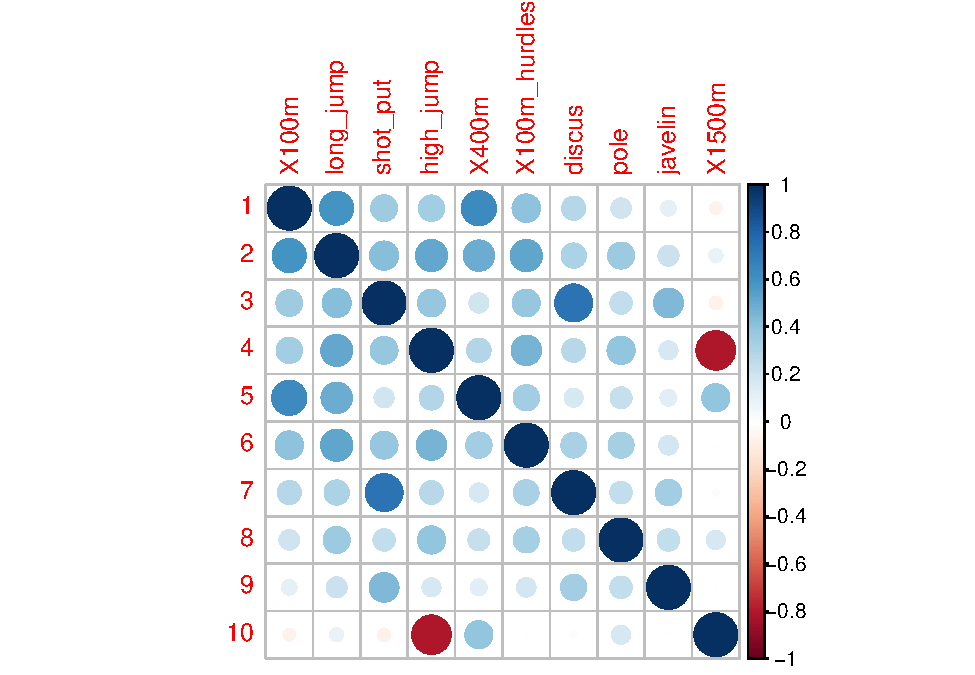
\includegraphics{hw2_files/figure-latex/unnamed-chunk-8-1.pdf} Repetimos
lo mismo para la segunda columna de nuestro data frame para realizar el
incizo d).

Proyección sobre \(1' = (1,1,1,1,1,1)\)

\begin{Shaded}
\begin{Highlighting}[]
\NormalTok{X2}\FloatTok{.3}
\end{Highlighting}
\end{Shaded}

\begin{verbatim}
## [1] 0.623 0.593 0.512 0.500 0.463 0.395
\end{verbatim}

\begin{Shaded}
\begin{Highlighting}[]
\NormalTok{(proy2 <-}\StringTok{ }\KeywordTok{proy}\NormalTok{(X2}\FloatTok{.3}\NormalTok{,unos))}
\end{Highlighting}
\end{Shaded}

\begin{verbatim}
## [1] 0.5143333 0.5143333 0.5143333 0.5143333 0.5143333 0.5143333
\end{verbatim}

Ahora calculamos el vector de desviacion. \(y_2 - \bar{x}_2\) y
verificamos su relacion con la desviacion estandar.

\begin{Shaded}
\begin{Highlighting}[]
\NormalTok{(d2}\FloatTok{.3}\NormalTok{ <-}\StringTok{ }\NormalTok{X2}\FloatTok{.3} \OperatorTok{-}\StringTok{ }\NormalTok{proy2)}
\end{Highlighting}
\end{Shaded}

\begin{verbatim}
## [1]  0.108666667  0.078666667 -0.002333333 -0.014333333 -0.051333333
## [6] -0.119333333
\end{verbatim}

\begin{Shaded}
\begin{Highlighting}[]
\KeywordTok{norm_vec}\NormalTok{(d2}\FloatTok{.3}\NormalTok{)}\OperatorTok{/}\KeywordTok{sqrt}\NormalTok{(}\DecValTok{5}\NormalTok{)}
\end{Highlighting}
\end{Shaded}

\begin{verbatim}
## [1] 0.08376555
\end{verbatim}

\begin{Shaded}
\begin{Highlighting}[]
\KeywordTok{sd}\NormalTok{(X2}\FloatTok{.3}\NormalTok{)}
\end{Highlighting}
\end{Shaded}

\begin{verbatim}
## [1] 0.08376555
\end{verbatim}

Por ultimo, realizamos la grafica del triangulo formado por \(y_2\)
\(\bar{x}_2\) y \(y_2 - \bar{x}_2\).

\begin{Shaded}
\begin{Highlighting}[]
\NormalTok{x2}\FloatTok{.3}\NormalTok{ <-}\StringTok{ }\NormalTok{X2}\FloatTok{.3}\NormalTok{[}\KeywordTok{c}\NormalTok{(}\DecValTok{1}\NormalTok{,}\DecValTok{2}\NormalTok{)]}
\NormalTok{x2.}\FloatTok{3.}\NormalTok{mean <-}\StringTok{ }\KeywordTok{proy}\NormalTok{(x2}\FloatTok{.3}\NormalTok{,}\KeywordTok{c}\NormalTok{(}\DecValTok{1}\NormalTok{,}\DecValTok{1}\NormalTok{))}
\NormalTok{d2 <-}\StringTok{ }\NormalTok{x2}\FloatTok{.3} \OperatorTok{-}\StringTok{ }\NormalTok{x2.}\FloatTok{3.}\NormalTok{mean}

\CommentTok{#normalizamos}
\NormalTok{x2}\FloatTok{.3}\NormalTok{ <-}\StringTok{ }\NormalTok{x2}\FloatTok{.3}\OperatorTok{/}\KeywordTok{norm_vec}\NormalTok{(x2}\FloatTok{.3}\NormalTok{)}
\NormalTok{x2.}\FloatTok{3.}\NormalTok{mean <-}\StringTok{ }\NormalTok{x2.}\FloatTok{3.}\NormalTok{mean}\OperatorTok{/}\KeywordTok{norm_vec}\NormalTok{(x2.}\FloatTok{3.}\NormalTok{mean)}
\NormalTok{d2 <-}\StringTok{ }\NormalTok{d2}\OperatorTok{/}\KeywordTok{norm_vec}\NormalTok{(d2)}
\NormalTok{data}\FloatTok{.3}\NormalTok{d <-}\KeywordTok{rbind}\NormalTok{(x2}\FloatTok{.3}\NormalTok{,x2.}\FloatTok{3.}\NormalTok{mean,d2)}
\NormalTok{x4 <-}\StringTok{ }\KeywordTok{as.array}\NormalTok{(data}\FloatTok{.3}\NormalTok{d[,}\DecValTok{1}\NormalTok{])}
\NormalTok{y4 <-}\StringTok{ }\KeywordTok{as.array}\NormalTok{(data}\FloatTok{.3}\NormalTok{d[,}\DecValTok{2}\NormalTok{])}
\KeywordTok{plot}\NormalTok{(x4,y4)}
\KeywordTok{polygon}\NormalTok{(x4,y4, }\DataTypeTok{border =} \StringTok{'green'}\NormalTok{)}
\end{Highlighting}
\end{Shaded}

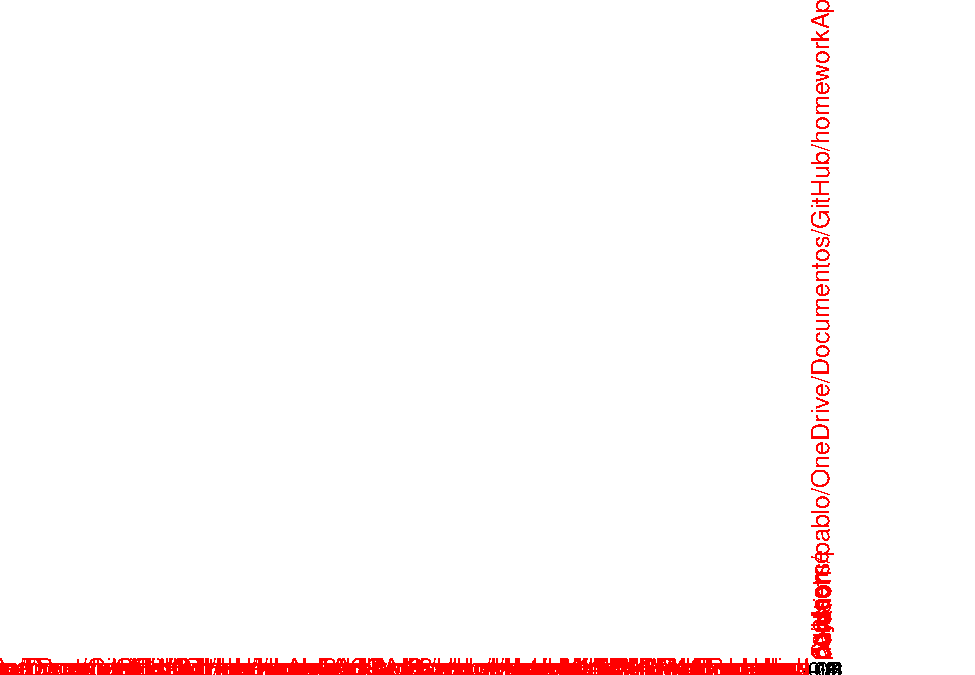
\includegraphics{hw2_files/figure-latex/unnamed-chunk-11-1.pdf} Para el
inciso e), graficaremos los dos vectores de desviación
\(y_1 - \bar{x}_1\) y \(y_2 - \bar{x}_2\). Dada la complejidad del
problema solo graficaremos las primeras dos entradas.

\begin{Shaded}
\begin{Highlighting}[]
\CommentTok{#intento 1) con vector de dos dimensions, el problema es que es el mismo d1 y d2}
\NormalTok{D1 <-}\StringTok{ }\KeywordTok{c}\NormalTok{(}\DecValTok{0}\NormalTok{,d1[}\DecValTok{1}\NormalTok{])}
\NormalTok{D2 <-}\StringTok{ }\KeywordTok{c}\NormalTok{(}\DecValTok{0}\NormalTok{,d1[}\DecValTok{2}\NormalTok{])}
\KeywordTok{plot}\NormalTok{(D1,D2)}
\KeywordTok{arrows}\NormalTok{(D1[}\DecValTok{1}\NormalTok{],D2[}\DecValTok{1}\NormalTok{],D1[}\DecValTok{2}\NormalTok{],D2[}\DecValTok{2}\NormalTok{])}
\end{Highlighting}
\end{Shaded}

\includegraphics{hw2_files/figure-latex/unnamed-chunk-12-1.pdf}

\begin{Shaded}
\begin{Highlighting}[]
\CommentTok{#intento 2) con solo las primeras dos entradas}
\NormalTok{D1}\FloatTok{.3}\NormalTok{ <-}\StringTok{ }\NormalTok{d1}\FloatTok{.3}\NormalTok{[}\KeywordTok{c}\NormalTok{(}\DecValTok{1}\NormalTok{,}\DecValTok{2}\NormalTok{)]}
\NormalTok{D2}\FloatTok{.3}\NormalTok{ <-}\StringTok{ }\NormalTok{d2}\FloatTok{.3}\NormalTok{[}\KeywordTok{c}\NormalTok{(}\DecValTok{1}\NormalTok{,}\DecValTok{2}\NormalTok{)]}
\NormalTok{D1}\FloatTok{.3}\NormalTok{ <-}\StringTok{ }\NormalTok{D1}\FloatTok{.3}\OperatorTok{/}\StringTok{ }\KeywordTok{norm_vec}\NormalTok{(D1}\FloatTok{.3}\NormalTok{)}
\NormalTok{D2}\FloatTok{.3}\NormalTok{ <-}\StringTok{ }\NormalTok{D2}\FloatTok{.3}\OperatorTok{/}\StringTok{ }\KeywordTok{norm_vec}\NormalTok{(D2}\FloatTok{.3}\NormalTok{)}
\NormalTok{D<-}\StringTok{ }\KeywordTok{rbind}\NormalTok{(D1}\FloatTok{.3}\NormalTok{,D2}\FloatTok{.3}\NormalTok{)}
\KeywordTok{plot}\NormalTok{(D[,}\DecValTok{1}\NormalTok{],D[,}\DecValTok{2}\NormalTok{],}\DataTypeTok{type=}\StringTok{"n"}\NormalTok{, }\DataTypeTok{xlim=}\KeywordTok{c}\NormalTok{(}\DecValTok{0}\NormalTok{, }\DecValTok{1}\NormalTok{), }\DataTypeTok{ylim=}\KeywordTok{c}\NormalTok{(}\DecValTok{0}\NormalTok{,}\DecValTok{1}\NormalTok{))}
\KeywordTok{arrows}\NormalTok{(}\DecValTok{0}\NormalTok{,}\DecValTok{0}\NormalTok{,}\DataTypeTok{x1 =}\NormalTok{ D[}\KeywordTok{c}\NormalTok{(}\DecValTok{1}\NormalTok{,}\DecValTok{1}\NormalTok{)],}\DataTypeTok{y1 =}\NormalTok{ D[}\KeywordTok{c}\NormalTok{(}\DecValTok{1}\NormalTok{,}\DecValTok{2}\NormalTok{)])}
\end{Highlighting}
\end{Shaded}

\includegraphics{hw2_files/figure-latex/unnamed-chunk-12-2.pdf} Para
calcular el angulo entre los dos vectores utilizaremos los vectores en
seis dimensiones originales y la siguiente formula.
\[ d_i'd_k = L_{d_i}L_{d_k}cos(\theta_{ik})\] por lo tanto
\[cos(\theta_{ik}) = \frac{d_i'd_k }{L_{d_i}L_{d_k}}\] de donde
\[\theta_{ik} = cos^{-1}(\frac{d_i'd_k }{L_{d_i}L_{d_k}})\]

\begin{Shaded}
\begin{Highlighting}[]
\NormalTok{v <-}\StringTok{ }\NormalTok{((}\KeywordTok{t}\NormalTok{(d1}\FloatTok{.3}\NormalTok{)}\OperatorTok\NormalTok{d2}\FloatTok{.3}\NormalTok{)[}\DecValTok{1}\NormalTok{]}\OperatorTok{/}\NormalTok{((}\KeywordTok{norm_vec}\NormalTok{(d1}\FloatTok{.3}\NormalTok{))}\OperatorTok{*}\NormalTok{(}\KeywordTok{norm_vec}\NormalTok{(d2}\FloatTok{.3}\NormalTok{))))}
\NormalTok{(theta <-}\StringTok{ }\KeywordTok{acos}\NormalTok{(v))}
\end{Highlighting}
\end{Shaded}

\begin{verbatim}
## [1] 0.4687649
\end{verbatim}

ahora para el inciso f) calcularemos la viaranza muestral generalizada.
Dado que se cumple que \(d_i'dj = nS_{ij}\) hacemos lo siguiente. Para
primero calcular \(S_n\)

\begin{Shaded}
\begin{Highlighting}[]
\CommentTok{#Duda si dividir entre 6 o 6-1}
\NormalTok{s1}\FloatTok{.3}\NormalTok{ <-}\StringTok{ }\NormalTok{(}\KeywordTok{t}\NormalTok{(d1}\FloatTok{.3}\NormalTok{)}\OperatorTok\NormalTok{d1}\FloatTok{.3}\NormalTok{)[}\DecValTok{1}\NormalTok{]}\OperatorTok{/}\NormalTok{(}\DecValTok{6-1}\NormalTok{)}
\NormalTok{s2}\FloatTok{.3}\NormalTok{ <-}\StringTok{ }\NormalTok{(}\KeywordTok{t}\NormalTok{(d2}\FloatTok{.3}\NormalTok{)}\OperatorTok\NormalTok{d2}\FloatTok{.3}\NormalTok{)[}\DecValTok{1}\NormalTok{]}\OperatorTok{/}\NormalTok{(}\DecValTok{6-1}\NormalTok{)}
\NormalTok{sc}\FloatTok{.3}\NormalTok{ <-}\StringTok{ }\NormalTok{(}\KeywordTok{t}\NormalTok{(d1}\FloatTok{.3}\NormalTok{)}\OperatorTok\NormalTok{d2}\FloatTok{.3}\NormalTok{)[}\DecValTok{1}\NormalTok{]}\OperatorTok{/}\NormalTok{(}\DecValTok{6-1}\NormalTok{)}

\NormalTok{Sn}\FloatTok{.3}\NormalTok{ <-}\StringTok{ }\KeywordTok{matrix}\NormalTok{(}\KeywordTok{c}\NormalTok{(s1}\FloatTok{.3}\NormalTok{,sc}\FloatTok{.3}\NormalTok{,sc}\FloatTok{.3}\NormalTok{,s2}\FloatTok{.3}\NormalTok{),}\DecValTok{2}\NormalTok{,}\DecValTok{2}\NormalTok{,}\DataTypeTok{byrow =} \OtherTok{TRUE}\NormalTok{)}
\KeywordTok{det}\NormalTok{(Sn}\FloatTok{.3}\NormalTok{)}
\end{Highlighting}
\end{Shaded}

\begin{verbatim}
## [1] 844182191
\end{verbatim}

\begin{Shaded}
\begin{Highlighting}[]
\CommentTok{# comparando con la obtenida por R}
\NormalTok{X3 <-}\StringTok{ }\KeywordTok{cbind}\NormalTok{(data3}\OperatorTok{$}\NormalTok{x1,data3}\OperatorTok{$}\NormalTok{x2)}
\NormalTok{S3 <-}\StringTok{ }\KeywordTok{cov}\NormalTok{(X3)}

\NormalTok{(}\KeywordTok{det}\NormalTok{(S3))}
\end{Highlighting}
\end{Shaded}

\begin{verbatim}
## [1] 844182191
\end{verbatim}

para el inciso g) calculamos la \(tr(S)\)

\begin{Shaded}
\begin{Highlighting}[]
\KeywordTok{sum}\NormalTok{(}\KeywordTok{diag}\NormalTok{(Sn}\FloatTok{.3}\NormalTok{))}
\end{Highlighting}
\end{Shaded}

\begin{verbatim}
## [1] 589443426354
\end{verbatim}

\#\#Ejercicio 4 4 Dibuja las elipsoides sólidas
\(\{{x|(x − \bar{x})'S^{-1}(x − \bar{x}) ≤ 1\}}\) para las tres matrices
siguientes y determina los valores de los ejes mayores y menores.
a)\[S = \left(\begin{array}{cc} 
5 & 4\\
4 & 5
\end{array}\right)\]\\
Asumimos que la media es cero, es decir \(\bar{x} = 0\). Esto hara que
nuestras elipses esten centradas en el origen. Los ejesY procedemos de
la siguiente forma.

\begin{Shaded}
\begin{Highlighting}[]
\NormalTok{S1 <-}\StringTok{ }\KeywordTok{matrix}\NormalTok{(}\KeywordTok{c}\NormalTok{(}\DecValTok{5}\NormalTok{,}\DecValTok{4}\NormalTok{,}\DecValTok{4}\NormalTok{,}\DecValTok{5}\NormalTok{),}\DataTypeTok{nrow =} \DecValTok{2}\NormalTok{, }\DataTypeTok{byrow =}\NormalTok{ T)}
\NormalTok{lambdas1 <-}\StringTok{ }\KeywordTok{eigen}\NormalTok{(S1)}\OperatorTok{$}\NormalTok{values}
\NormalTok{(eje.mayor <-}\StringTok{ }\KeywordTok{sqrt}\NormalTok{(}\KeywordTok{max}\NormalTok{(lambdas1)))}
\end{Highlighting}
\end{Shaded}

\begin{verbatim}
## [1] 3
\end{verbatim}

\begin{Shaded}
\begin{Highlighting}[]
\NormalTok{(eje.menor <-}\StringTok{ }\KeywordTok{sqrt}\NormalTok{(}\KeywordTok{min}\NormalTok{(lambdas1)))}
\end{Highlighting}
\end{Shaded}

\begin{verbatim}
## [1] 1
\end{verbatim}

\begin{Shaded}
\begin{Highlighting}[]
\NormalTok{mu <-}\StringTok{ }\KeywordTok{c}\NormalTok{(}\DecValTok{0}\NormalTok{, }\DecValTok{0}\NormalTok{)  }\CommentTok{#vector medias}
\NormalTok{DC <-}\StringTok{ }\KeywordTok{chol}\NormalTok{(S1) }\CommentTok{# descomposición de Cholesky}
\NormalTok{angl <-}\StringTok{ }\KeywordTok{seq}\NormalTok{(}\DecValTok{0}\NormalTok{, }\DecValTok{2}\OperatorTok{*}\NormalTok{pi, }\DataTypeTok{length.out=}\DecValTok{200}\NormalTok{) }
\NormalTok{elipse.esc <-}\StringTok{ }\DecValTok{1} \OperatorTok{*}\StringTok{ }\KeywordTok{cbind}\NormalTok{(}\KeywordTok{cos}\NormalTok{(angl), }\KeywordTok{sin}\NormalTok{(angl)) }\OperatorTok\StringTok{ }\NormalTok{DC }\CommentTok{# elipse escalada}
\NormalTok{elipseCentro <-}\StringTok{ }\KeywordTok{sweep}\NormalTok{(elipse.esc, }\DecValTok{2}\NormalTok{, mu, }\StringTok{"+"}\NormalTok{) }\CommentTok{# centramos en la media}
\KeywordTok{plot}\NormalTok{(elipseCentro, }\DataTypeTok{type=}\StringTok{"l"}\NormalTok{, }\DataTypeTok{lwd=}\DecValTok{2}\NormalTok{, }\DataTypeTok{asp=}\DecValTok{1}\NormalTok{, }\DataTypeTok{xlab=}\StringTok{"x"}\NormalTok{,}\DataTypeTok{ylab=}\StringTok{"y"}\NormalTok{, }\DataTypeTok{main=}\StringTok{"S1"}\NormalTok{)}
\KeywordTok{points}\NormalTok{(mu[}\DecValTok{1}\NormalTok{], mu[}\DecValTok{2}\NormalTok{], }\DataTypeTok{pch=}\DecValTok{4}\NormalTok{, }\DataTypeTok{lwd=}\DecValTok{2}\NormalTok{, }\DataTypeTok{col=}\StringTok{"red"}\NormalTok{) }
\CommentTok{#Ejes en la dirección de las componentes principales:}
\NormalTok{Sinv <-}\StringTok{ }\KeywordTok{solve}\NormalTok{(S1) }\CommentTok{#inversa de la matriz de covarianzas}
\NormalTok{DE <-}\StringTok{ }\KeywordTok{eigen}\NormalTok{(Sinv) }\CommentTok{#descomposición espectral de Sinv}
\NormalTok{s1 <-}\StringTok{ }\DecValTok{2} \CommentTok{#factor de escala}
\NormalTok{s2 <-}\StringTok{ }\DecValTok{1}
\KeywordTok{arrows}\NormalTok{(}\DataTypeTok{x0 =}\NormalTok{ mu[}\DecValTok{1}\NormalTok{], }\DataTypeTok{y0 =}\NormalTok{ mu[}\DecValTok{2}\NormalTok{],}
\DataTypeTok{x1 =}\NormalTok{ mu[}\DecValTok{1}\NormalTok{] }\OperatorTok{+}\StringTok{ }\NormalTok{s2}\OperatorTok{*}\NormalTok{DE}\OperatorTok{$}\NormalTok{vectors[}\DecValTok{1}\NormalTok{,}\DecValTok{1}\NormalTok{], }\DataTypeTok{y1 =}\NormalTok{ mu[}\DecValTok{2}\NormalTok{] }\OperatorTok{+}\StringTok{ }\NormalTok{s2}\OperatorTok{*}\NormalTok{DE}\OperatorTok{$}\NormalTok{vectors[}\DecValTok{2}\NormalTok{,}\DecValTok{1}\NormalTok{], }\DataTypeTok{length =} \FloatTok{0.1}\NormalTok{, }\DataTypeTok{col =} \StringTok{"red"}\NormalTok{)}
\KeywordTok{arrows}\NormalTok{(}\DataTypeTok{x0 =}\NormalTok{ mu[}\DecValTok{1}\NormalTok{], }\DataTypeTok{y0 =}\NormalTok{ mu[}\DecValTok{2}\NormalTok{],}
\DataTypeTok{x1 =}\NormalTok{ mu[}\DecValTok{1}\NormalTok{] }\OperatorTok{+}\StringTok{ }\NormalTok{s1}\OperatorTok{*}\NormalTok{DE}\OperatorTok{$}\NormalTok{vectors[}\DecValTok{1}\NormalTok{,}\DecValTok{2}\NormalTok{], }\DataTypeTok{y1 =}\NormalTok{ mu[}\DecValTok{2}\NormalTok{] }\OperatorTok{+}\StringTok{ }\NormalTok{s1}\OperatorTok{*}\NormalTok{DE}\OperatorTok{$}\NormalTok{vectors[}\DecValTok{2}\NormalTok{,}\DecValTok{2}\NormalTok{], }\DataTypeTok{length =} \FloatTok{0.1}\NormalTok{, }\DataTypeTok{col =} \StringTok{"red"}\NormalTok{)}
\end{Highlighting}
\end{Shaded}

\includegraphics{hw2_files/figure-latex/unnamed-chunk-16-1.pdf} De donde
el eje mayor es 3 y el menor es 1.

b)\[S = \left(\begin{array}{cc} 
5 & -4\\
-4 & 5
\end{array}\right)\]

\begin{Shaded}
\begin{Highlighting}[]
\NormalTok{S2 <-}\StringTok{ }\KeywordTok{matrix}\NormalTok{(}\KeywordTok{c}\NormalTok{(}\DecValTok{5}\NormalTok{,}\OperatorTok{-}\DecValTok{4}\NormalTok{,}\OperatorTok{-}\DecValTok{4}\NormalTok{,}\DecValTok{5}\NormalTok{),}\DataTypeTok{nrow =} \DecValTok{2}\NormalTok{, }\DataTypeTok{byrow =}\NormalTok{ T)}
\NormalTok{lambdas2 <-}\StringTok{ }\KeywordTok{eigen}\NormalTok{(S2)}\OperatorTok{$}\NormalTok{values}
\NormalTok{(eje.mayor <-}\StringTok{ }\KeywordTok{sqrt}\NormalTok{(}\KeywordTok{max}\NormalTok{(lambdas2)))}
\end{Highlighting}
\end{Shaded}

\begin{verbatim}
## [1] 3
\end{verbatim}

\begin{Shaded}
\begin{Highlighting}[]
\NormalTok{(eje.menor <-}\StringTok{ }\KeywordTok{sqrt}\NormalTok{(}\KeywordTok{min}\NormalTok{(lambdas2)))}
\end{Highlighting}
\end{Shaded}

\begin{verbatim}
## [1] 1
\end{verbatim}

\begin{Shaded}
\begin{Highlighting}[]
\NormalTok{mu <-}\StringTok{ }\KeywordTok{c}\NormalTok{(}\DecValTok{0}\NormalTok{, }\DecValTok{0}\NormalTok{)  }\CommentTok{#vector medias}
\NormalTok{DC <-}\StringTok{ }\KeywordTok{chol}\NormalTok{(S2) }\CommentTok{# descomposición de Cholesky}
\NormalTok{angl <-}\StringTok{ }\KeywordTok{seq}\NormalTok{(}\DecValTok{0}\NormalTok{, }\DecValTok{2}\OperatorTok{*}\NormalTok{pi, }\DataTypeTok{length.out=}\DecValTok{200}\NormalTok{) }
\NormalTok{elipse.esc <-}\StringTok{ }\DecValTok{1} \OperatorTok{*}\StringTok{ }\KeywordTok{cbind}\NormalTok{(}\KeywordTok{cos}\NormalTok{(angl), }\KeywordTok{sin}\NormalTok{(angl)) }\OperatorTok\StringTok{ }\NormalTok{DC }\CommentTok{# elipse escalada}
\NormalTok{elipseCentro <-}\StringTok{ }\KeywordTok{sweep}\NormalTok{(elipse.esc, }\DecValTok{2}\NormalTok{, mu, }\StringTok{"+"}\NormalTok{) }\CommentTok{# centramos en la media}
\KeywordTok{plot}\NormalTok{(elipseCentro, }\DataTypeTok{type=}\StringTok{"l"}\NormalTok{, }\DataTypeTok{lwd=}\DecValTok{2}\NormalTok{, }\DataTypeTok{asp=}\DecValTok{1}\NormalTok{, }\DataTypeTok{xlab=}\StringTok{"x"}\NormalTok{,}\DataTypeTok{ylab=}\StringTok{"y"}\NormalTok{, }\DataTypeTok{main=}\StringTok{"b)"}\NormalTok{)}
\KeywordTok{points}\NormalTok{(mu[}\DecValTok{1}\NormalTok{], mu[}\DecValTok{2}\NormalTok{], }\DataTypeTok{pch=}\DecValTok{4}\NormalTok{, }\DataTypeTok{lwd=}\DecValTok{2}\NormalTok{, }\DataTypeTok{col=}\StringTok{"red"}\NormalTok{) }
\CommentTok{#Ejes en la dirección de las componentes principales:}
\NormalTok{Sinv <-}\StringTok{ }\KeywordTok{solve}\NormalTok{(S1) }\CommentTok{#inversa de la matriz de covarianzas}
\NormalTok{DE <-}\StringTok{ }\KeywordTok{eigen}\NormalTok{(Sinv) }\CommentTok{#descomposición espectral de Sinv}
\NormalTok{s1 <-}\StringTok{ }\DecValTok{2} \CommentTok{#factor de escala}
\NormalTok{s2 <-}\StringTok{ }\DecValTok{1}
\KeywordTok{arrows}\NormalTok{(}\DataTypeTok{x0 =}\NormalTok{ mu[}\DecValTok{1}\NormalTok{], }\DataTypeTok{y0 =}\NormalTok{ mu[}\DecValTok{2}\NormalTok{],}
\DataTypeTok{x1 =}\NormalTok{ mu[}\DecValTok{1}\NormalTok{] }\OperatorTok{+}\StringTok{ }\NormalTok{s1}\OperatorTok{*}\NormalTok{DE}\OperatorTok{$}\NormalTok{vectors[}\DecValTok{1}\NormalTok{,}\DecValTok{1}\NormalTok{], }\DataTypeTok{y1 =}\NormalTok{ mu[}\DecValTok{2}\NormalTok{] }\OperatorTok{+}\StringTok{ }\NormalTok{s1}\OperatorTok{*}\NormalTok{DE}\OperatorTok{$}\NormalTok{vectors[}\DecValTok{2}\NormalTok{,}\DecValTok{1}\NormalTok{], }\DataTypeTok{length =} \FloatTok{0.1}\NormalTok{, }\DataTypeTok{col =} \StringTok{"red"}\NormalTok{)}
\KeywordTok{arrows}\NormalTok{(}\DataTypeTok{x0 =}\NormalTok{ mu[}\DecValTok{1}\NormalTok{], }\DataTypeTok{y0 =}\NormalTok{ mu[}\DecValTok{2}\NormalTok{],}
\DataTypeTok{x1 =}\NormalTok{ mu[}\DecValTok{1}\NormalTok{] }\OperatorTok{+}\StringTok{ }\NormalTok{s2}\OperatorTok{*}\NormalTok{DE}\OperatorTok{$}\NormalTok{vectors[}\DecValTok{1}\NormalTok{,}\DecValTok{2}\NormalTok{], }\DataTypeTok{y1 =}\NormalTok{ mu[}\DecValTok{2}\NormalTok{] }\OperatorTok{+}\StringTok{ }\NormalTok{s2}\OperatorTok{*}\NormalTok{DE}\OperatorTok{$}\NormalTok{vectors[}\DecValTok{2}\NormalTok{,}\DecValTok{2}\NormalTok{], }\DataTypeTok{length =} \FloatTok{0.1}\NormalTok{, }\DataTypeTok{col =} \StringTok{"red"}\NormalTok{)}
\end{Highlighting}
\end{Shaded}

\includegraphics{hw2_files/figure-latex/unnamed-chunk-17-1.pdf} Al igual
que en el inciso anterior el eje mayor es 3 y el menor es 1.

c)\[S = \left(\begin{array}{cc} 
3 & 0\\
3 & 3
\end{array}\right)\]

\begin{Shaded}
\begin{Highlighting}[]
\NormalTok{S3 <-}\StringTok{ }\KeywordTok{matrix}\NormalTok{(}\KeywordTok{c}\NormalTok{(}\DecValTok{3}\NormalTok{,}\DecValTok{0}\NormalTok{,}\DecValTok{0}\NormalTok{,}\DecValTok{3}\NormalTok{),}\DataTypeTok{nrow =} \DecValTok{2}\NormalTok{, }\DataTypeTok{byrow =}\NormalTok{ T)}
\NormalTok{lambdas3 <-}\StringTok{ }\KeywordTok{eigen}\NormalTok{(S3)}\OperatorTok{$}\NormalTok{values}
\NormalTok{(eje.mayor <-}\StringTok{ }\KeywordTok{sqrt}\NormalTok{(}\KeywordTok{max}\NormalTok{(lambdas3)))}
\end{Highlighting}
\end{Shaded}

\begin{verbatim}
## [1] 1.732051
\end{verbatim}

\begin{Shaded}
\begin{Highlighting}[]
\NormalTok{(eje.menor <-}\StringTok{ }\KeywordTok{sqrt}\NormalTok{(}\KeywordTok{min}\NormalTok{(lambdas3)))}
\end{Highlighting}
\end{Shaded}

\begin{verbatim}
## [1] 1.732051
\end{verbatim}

\begin{Shaded}
\begin{Highlighting}[]
\NormalTok{mu <-}\StringTok{ }\KeywordTok{c}\NormalTok{(}\DecValTok{0}\NormalTok{, }\DecValTok{0}\NormalTok{)  }\CommentTok{#vector medias}
\NormalTok{DC <-}\StringTok{ }\KeywordTok{chol}\NormalTok{(S3) }\CommentTok{# descomposición de Cholesky}
\NormalTok{angl <-}\StringTok{ }\KeywordTok{seq}\NormalTok{(}\DecValTok{0}\NormalTok{, }\DecValTok{2}\OperatorTok{*}\NormalTok{pi, }\DataTypeTok{length.out=}\DecValTok{200}\NormalTok{) }
\NormalTok{elipse.esc <-}\StringTok{ }\DecValTok{1} \OperatorTok{*}\StringTok{ }\KeywordTok{cbind}\NormalTok{(}\KeywordTok{cos}\NormalTok{(angl), }\KeywordTok{sin}\NormalTok{(angl)) }\OperatorTok\StringTok{ }\NormalTok{DC }\CommentTok{# elipse escalada}
\NormalTok{elipseCentro <-}\StringTok{ }\KeywordTok{sweep}\NormalTok{(elipse.esc, }\DecValTok{2}\NormalTok{, mu, }\StringTok{"+"}\NormalTok{) }\CommentTok{# centramos en la media}
\KeywordTok{plot}\NormalTok{(elipseCentro, }\DataTypeTok{type=}\StringTok{"l"}\NormalTok{, }\DataTypeTok{lwd=}\DecValTok{2}\NormalTok{, }\DataTypeTok{asp=}\DecValTok{1}\NormalTok{, }\DataTypeTok{xlab=}\StringTok{"x"}\NormalTok{,}\DataTypeTok{ylab=}\StringTok{"y"}\NormalTok{, }\DataTypeTok{main=}\StringTok{"c)"}\NormalTok{)}
\KeywordTok{points}\NormalTok{(mu[}\DecValTok{1}\NormalTok{], mu[}\DecValTok{2}\NormalTok{], }\DataTypeTok{pch=}\DecValTok{4}\NormalTok{, }\DataTypeTok{lwd=}\DecValTok{2}\NormalTok{, }\DataTypeTok{col=}\StringTok{"red"}\NormalTok{) }
\CommentTok{#Ejes en la dirección de las componentes principales:}
\NormalTok{Sinv <-}\StringTok{ }\KeywordTok{solve}\NormalTok{(S1) }\CommentTok{#inversa de la matriz de covarianzas}
\NormalTok{DE <-}\StringTok{ }\KeywordTok{eigen}\NormalTok{(Sinv) }\CommentTok{#descomposición espectral de Sinv}
\NormalTok{s <-}\StringTok{ }\FloatTok{1.5} \CommentTok{#factor de escala}
\KeywordTok{arrows}\NormalTok{(}\DataTypeTok{x0 =}\NormalTok{ mu[}\DecValTok{1}\NormalTok{], }\DataTypeTok{y0 =}\NormalTok{ mu[}\DecValTok{2}\NormalTok{],}
\DataTypeTok{x1 =}\NormalTok{ mu[}\DecValTok{1}\NormalTok{] }\OperatorTok{+}\StringTok{ }\NormalTok{s}\OperatorTok{*}\NormalTok{DE}\OperatorTok{$}\NormalTok{vectors[}\DecValTok{1}\NormalTok{,}\DecValTok{1}\NormalTok{], }\DataTypeTok{y1 =}\NormalTok{ mu[}\DecValTok{2}\NormalTok{] }\OperatorTok{+}\StringTok{ }\NormalTok{s}\OperatorTok{*}\NormalTok{DE}\OperatorTok{$}\NormalTok{vectors[}\DecValTok{2}\NormalTok{,}\DecValTok{1}\NormalTok{], }\DataTypeTok{length =} \FloatTok{0.1}\NormalTok{, }\DataTypeTok{col =} \StringTok{"red"}\NormalTok{)}
\KeywordTok{arrows}\NormalTok{(}\DataTypeTok{x0 =}\NormalTok{ mu[}\DecValTok{1}\NormalTok{], }\DataTypeTok{y0 =}\NormalTok{ mu[}\DecValTok{2}\NormalTok{],}
\DataTypeTok{x1 =}\NormalTok{ mu[}\DecValTok{1}\NormalTok{] }\OperatorTok{+}\StringTok{ }\NormalTok{s}\OperatorTok{*}\NormalTok{DE}\OperatorTok{$}\NormalTok{vectors[}\DecValTok{1}\NormalTok{,}\DecValTok{2}\NormalTok{], }\DataTypeTok{y1 =}\NormalTok{ mu[}\DecValTok{2}\NormalTok{] }\OperatorTok{+}\StringTok{ }\NormalTok{s}\OperatorTok{*}\NormalTok{DE}\OperatorTok{$}\NormalTok{vectors[}\DecValTok{2}\NormalTok{,}\DecValTok{2}\NormalTok{], }\DataTypeTok{length =} \FloatTok{0.1}\NormalTok{, }\DataTypeTok{col =} \StringTok{"red"}\NormalTok{)}
\end{Highlighting}
\end{Shaded}

\includegraphics{hw2_files/figure-latex/unnamed-chunk-18-1.pdf} En este
caso tanto el eje menor como el mayor son 1.7 \#\#Ejercicio 5

Leyendo la base de datos.

\begin{Shaded}
\begin{Highlighting}[]
\CommentTok{#read databse}
\NormalTok{file <-}\StringTok{ 'INEGIConstruccion2017.csv'}
\NormalTok{df_inegi <-}\StringTok{ }\KeywordTok{read.csv}\NormalTok{(}\DataTypeTok{file =} \KeywordTok{paste}\NormalTok{(file,}\DataTypeTok{sep =} \StringTok{""}\NormalTok{),}\DataTypeTok{header =}\NormalTok{ T,}\DataTypeTok{skip =} \DecValTok{0}\NormalTok{) }\CommentTok{#skip lines}
\end{Highlighting}
\end{Shaded}

Observamos que las variables están colocadas de manera continua sobre
todas las columnas, son 215 variables. Queremos hacer una matriz \(X\)
donde sus variables sean las mencionadas anteriormente y sus
oobservaciones sean los estados para enero del 2017.

Además, notamos lo siguiente: - Hay columnas faltantes. - Entre cada
variable, hay un \emph{total nacional}. (Se optará por eliminarlo, ya
que produce colinealidad). - De la variable \textbf{Valor de producción
generado \ldots{}}, sólo hay \emph{16} observaciones. Por lo que quitar
los renglones \emph{NO} es opción. Se hará un remuestreo con reemplazo
para asignar el valor de las variables.

\hypertarget{a.-x-configurada-para-operar.}{%
\subsubsection{\texorpdfstring{5a. \(X\) configurada para
operar.}{5a. X configurada para operar.}}\label{a.-x-configurada-para-operar.}}

Se limpiará a continuación la base de datos de forma manual, debido a
que no hay un patrón definido.

\begin{Shaded}
\begin{Highlighting}[]
\KeywordTok{set.seed}\NormalTok{(}\DecValTok{42}\NormalTok{)}
\CommentTok{#copy raw data}
\NormalTok{file2 <-}\StringTok{ 'inegiClean.csv'}

\CommentTok{#clean}
\NormalTok{df_raw <-}\StringTok{ }\KeywordTok{read.csv}\NormalTok{(file2,}\DataTypeTok{header =} \OtherTok{FALSE}\NormalTok{)}
\NormalTok{df_raw <-}\StringTok{ }\KeywordTok{as.matrix}\NormalTok{(df_raw)}

\CommentTok{#data is transposed}
\NormalTok{df_raw <-}\StringTok{ }\KeywordTok{t}\NormalTok{(df_raw)}
\NormalTok{df_raw[}\DecValTok{17}\OperatorTok{:}\DecValTok{32}\NormalTok{,}\DecValTok{2}\NormalTok{] <-}\StringTok{ }\KeywordTok{sample}\NormalTok{(df_raw[}\DecValTok{1}\OperatorTok{:}\DecValTok{16}\NormalTok{,}\DecValTok{2}\NormalTok{], }\DataTypeTok{size =} \DecValTok{16}\NormalTok{, }\DataTypeTok{replace =}\NormalTok{ T)}
\NormalTok{X <-}\StringTok{ }\NormalTok{df_raw}

\CommentTok{#look}
\KeywordTok{tail}\NormalTok{(X)}
\end{Highlighting}
\end{Shaded}

\begin{verbatim}
##         [,1]      [,2]     [,3]     [,4]     [,5]   [,6]    [,7]
## V27 2261.705 3144478.7 1716.063 1169.822  501.094 45.147 545.642
## V28 6176.806 1404806.6 5224.554 4208.895  950.857 64.802 952.252
## V29  268.718  717169.8  268.210  200.665   57.040 10.505   0.508
## V30 6582.393  533582.3 6226.744 5041.573 1113.837 71.334 355.649
## V31 3423.691 2232549.7 3310.421 2572.381  708.740 29.300 113.270
## V32 1510.317 1059265.3 1495.929 1273.993  208.743 13.193  14.388
\end{verbatim}

\#\#\#5.b Calculate the mean vector and the variance and covariance
matrix

\begin{Shaded}
\begin{Highlighting}[]
\NormalTok{mean_vec <-}\StringTok{ }\KeywordTok{colMeans}\NormalTok{(X)}
\NormalTok{Sprime <-}\StringTok{ }\KeywordTok{cov}\NormalTok{(X)}

\KeywordTok{cat}\NormalTok{(}\StringTok{"}\CharTok{\textbackslash{}n}\StringTok{ Vector de medias}\CharTok{\textbackslash{}n}\StringTok{"}\NormalTok{)}
\end{Highlighting}
\end{Shaded}

\begin{verbatim}
## 
##  Vector de medias
\end{verbatim}

\begin{Shaded}
\begin{Highlighting}[]
\KeywordTok{kable}\NormalTok{(mean_vec,}\DataTypeTok{caption =} \StringTok{"Vector de medias"}\NormalTok{, }\DataTypeTok{digits =} \DecValTok{3}\NormalTok{)}
\end{Highlighting}
\end{Shaded}

\begin{longtable}[]{@{}r@{}}
\caption{Vector de medias}\tabularnewline
\toprule
x\tabularnewline
\midrule
\endfirsthead
\toprule
x\tabularnewline
\midrule
\endhead
4045.648\tabularnewline
1125180.444\tabularnewline
3366.957\tabularnewline
2642.589\tabularnewline
673.024\tabularnewline
51.344\tabularnewline
678.692\tabularnewline
\bottomrule
\end{longtable}

\begin{Shaded}
\begin{Highlighting}[]
\KeywordTok{cat}\NormalTok{(}\StringTok{"}\CharTok{\textbackslash{}n}\StringTok{ Matriz de var y cov}\CharTok{\textbackslash{}n}\StringTok{"}\NormalTok{)}
\end{Highlighting}
\end{Shaded}

\begin{verbatim}
## 
##  Matriz de var y cov
\end{verbatim}

\begin{Shaded}
\begin{Highlighting}[]
\KeywordTok{kable}\NormalTok{(Sprime, }\DataTypeTok{col.names =} \KeywordTok{c}\NormalTok{(}\StringTok{"X1"}\NormalTok{,}\StringTok{"X2"}\NormalTok{,}\StringTok{"X3"}\NormalTok{,}\StringTok{"X4"}\NormalTok{,}\StringTok{"X5"}\NormalTok{,}\StringTok{"X6"}\NormalTok{,}\StringTok{"X7"}\NormalTok{), }\DataTypeTok{digits =} \DecValTok{3}\NormalTok{)}
\end{Highlighting}
\end{Shaded}

\begin{longtable}[]{@{}rrrrrrr@{}}
\toprule
X1 & X2 & X3 & X4 & X5 & X6 & X7\tabularnewline
\midrule
\endhead
12302808.82 & 791597446 & 8156502.07 & 6418338.7 & 1659753.37 &
78409.975 & 4146306.75\tabularnewline
791597446.02 & 665503788827 & 599330930.44 & 380592172.0 & 203160295.91
& 15578462.578 & 192266515.57\tabularnewline
8156502.07 & 599330930 & 5877226.85 & 4685110.3 & 1138165.49 & 53951.050
& 2279275.21\tabularnewline
6418338.72 & 380592172 & 4685110.32 & 3795459.8 & 850416.39 & 39234.095
& 1733228.40\tabularnewline
1659753.37 & 203160296 & 1138165.49 & 850416.4 & 274187.77 & 13561.327 &
521587.89\tabularnewline
78409.98 & 15578463 & 53951.05 & 39234.1 & 13561.33 & 1155.627 &
24458.92\tabularnewline
4146306.75 & 192266516 & 2279275.21 & 1733228.4 & 521587.89 & 24458.925
& 1867031.54\tabularnewline
\bottomrule
\end{longtable}

\hypertarget{c.-verificar-dets-prod_i17s2-textdetr}{%
\subsubsection{\texorpdfstring{5c. Verificar det(\(S\)) =
\(\prod_{i=1}^{7}s^{2} \text{det}(R)\)}{5c. Verificar det(S) = \textbackslash prod\_\{i=1\}\^{}\{7\}s\^{}\{2\} \textbackslash text\{det\}(R)}}\label{c.-verificar-dets-prod_i17s2-textdetr}}

\begin{Shaded}
\begin{Highlighting}[]
\NormalTok{detS <-}\StringTok{ }\KeywordTok{det}\NormalTok{(Sprime)}

\CommentTok{#prove det}
\NormalTok{prodaux <-}\StringTok{ }\DecValTok{1}

\CommentTok{#measure vars}
\NormalTok{Rprime <-}\StringTok{ }\KeywordTok{cor}\NormalTok{(X) }\CommentTok{#corr matrix}
\NormalTok{n <-}\StringTok{ }\KeywordTok{ncol}\NormalTok{(X) }\CommentTok{#number of vars}
\NormalTok{D <-}\StringTok{ }\KeywordTok{diag}\NormalTok{(}\DataTypeTok{x =} \KeywordTok{eigen}\NormalTok{(Sprime)}\OperatorTok{$}\NormalTok{values,)}

\ControlFlowTok{for}\NormalTok{(i }\ControlFlowTok{in} \DecValTok{1}\OperatorTok{:}\NormalTok{n)}
\NormalTok{  prodaux <-}\StringTok{ }\NormalTok{prodaux }\OperatorTok{*}\StringTok{ }\NormalTok{D[i,i] }\OperatorTok{*}\StringTok{ }\KeywordTok{det}\NormalTok{(Rprime) }
\end{Highlighting}
\end{Shaded}

\#\#Ejercicio 6

Sea \(\underline{X} \sim \mathcal{N}_{3}(\underline{\mu},\Sigma)\) con
\(\underline{\mu}\) y \(\Sigma\) definidas como en la tarea. Determinar
cuales de las sig vars son independientes y porqué:

\begin{itemize}
\tightlist
\item
  \(X_{1} \ \text{y} \ X_{2}\): \textbf{Dependientes}, debido a que la
  covarianza entre ellas es distinta de cero.
\item
  \(X{2} \ \text{y} \ X_{3}\): \textbf{Independientes}, ya que la
  covarianza entre ellas es cero.
\item
  \((X_{1},X_{2}) \ \text{y} \ X_{3}\): \textbf{Independientes} ya que
  el bloque de la matriz \(\Sigma\) para \(X_{1,2} \ \text{y} \  X_{3}\)
  tiene ceros en los traingulos superiores e inferiores.
\item
  \(\frac{(X_{1} +X_{2})}{2} \ \text{y} \ X_{3}\):
  \textbf{Independientes}, por el inciso anterior.
\item
  \(X_{2} \ \text{y} \ X_{2} - \frac{5}{2}X_{1} - X_{3}\):
  \textbf{Dependientes}. Pues ambas variables \emph{dependen} del valor
  que tome \(X_{2}\).
\end{itemize}

\#\#Ejercicio 7 7. Sea \(X \sim N(\mu,\Sigma)\) con \[\mu' = (2,-3,1)\]
y \[\Sigma = \left(\begin{array}{cc} 
1 & 1 & 1\\
1 & 3 & 2 \\
1 & 2 & 2
\end{array}\right)\]

\begin{enumerate}
\def\labelenumi{\alph{enumi})}
\tightlist
\item
  Encuentra la distribucion de \(3X_1 - 2X_2 + X_3\)
\end{enumerate}

Dado que \(X \sim N\), sabemos que sus marginales tambien lo seran.
Tambien podemos afirmar que cualquier combinacion lineal sigue tambien
una distribucion normal. Para resolver este inciso utilizamos la
siguiente fomula. \[ a'X \sim N(a'\mu, a'\Sigma a)\] Por lo cual
obtenemos la media y varianza de la siguiente manera.

\begin{Shaded}
\begin{Highlighting}[]
\NormalTok{v =}\StringTok{ }\KeywordTok{c}\NormalTok{(}\DecValTok{3}\NormalTok{,}\OperatorTok{-}\DecValTok{2}\NormalTok{,}\DecValTok{1}\NormalTok{)}
\NormalTok{mu}\FloatTok{.7}\NormalTok{ <-}\StringTok{ }\KeywordTok{c}\NormalTok{(}\DecValTok{2}\NormalTok{,}\OperatorTok{-}\DecValTok{3}\NormalTok{,}\DecValTok{1}\NormalTok{)}
\NormalTok{s}\FloatTok{.7}\NormalTok{ <-}\StringTok{ }\KeywordTok{matrix}\NormalTok{(}\KeywordTok{c}\NormalTok{(}\DecValTok{1}\NormalTok{,}\DecValTok{1}\NormalTok{,}\DecValTok{1}\NormalTok{,}\DecValTok{1}\NormalTok{,}\DecValTok{3}\NormalTok{,}\DecValTok{2}\NormalTok{,}\DecValTok{1}\NormalTok{,}\DecValTok{2}\NormalTok{,}\DecValTok{2}\NormalTok{), }\DataTypeTok{nrow =} \DecValTok{3}\NormalTok{, }\DataTypeTok{ncol =} \DecValTok{3}\NormalTok{, }\DataTypeTok{byrow =} \OtherTok{TRUE}\NormalTok{)}
\NormalTok{(MU}\FloatTok{.7}\NormalTok{ <-}\StringTok{ }\KeywordTok{as.numeric}\NormalTok{(}\KeywordTok{t}\NormalTok{(v)}\OperatorTok\NormalTok{mu}\FloatTok{.7}\NormalTok{))}
\end{Highlighting}
\end{Shaded}

\begin{verbatim}
## [1] 13
\end{verbatim}

\begin{Shaded}
\begin{Highlighting}[]
\NormalTok{(S}\FloatTok{.7}\NormalTok{ <-}\StringTok{ }\KeywordTok{as.numeric}\NormalTok{(}\KeywordTok{t}\NormalTok{(v)}\OperatorTok\NormalTok{s}\FloatTok{.7}\OperatorTok\NormalTok{v))}
\end{Highlighting}
\end{Shaded}

\begin{verbatim}
## [1] 9
\end{verbatim}

Por lo tanto \(3X_1 - 2X_2 + X_3 \sim N(13,9)\)

\begin{enumerate}
\def\labelenumi{\alph{enumi})}
\setcounter{enumi}{1}
\tightlist
\item
  Encontrar un vector \(a\) tal que \(X_2\) y \(X_2 - a'(X_1,X_2)'\)
  sean independientes.
\end{enumerate}

Para resolver esto, basta con encontrar \(a\epsilon \Re^2\) tal que la
covarianza de \(X_2\) y \(X_2 - a'(X_1,X2)'\) sea cero.
\[\begin{array}{l}
cov(X_2,X_2 - a'(X_1,X_2)') = cov(X_2, X_2 - a_1X_1 + a_2X_2)\\
= cov(X_2,X_2) - a_1cov(X_1,X_2) - a_2cov(X_1,X_2)\\
= S_{22} -a_1S_{12} - a_2S_{22} 
= 3 -a_1 - 3a_2
\end{array}\]

Por lo tanto \[cov(X_2,X_2 - a'(X_1,X_2)') = 0 \]
\[\Leftrightarrow  3 -a_1 - 3a_2 = 0\] \[\Leftrightarrow  a_1+3a_2 = 3\]
Para lo cual existe toda una recta de combinaciones que cumple estas
condiciones. Basta con tomar \[\begin{array}{l}
a_1 = 0 \\
a_2 = 1
\end{array}\] \#\#Ejercicio 8

Sea \(y_{i} = Ax_{i} + b, \quad i = 1,\dots,n\), mostrar que

\hypertarget{i-bary-abarx-b}{%
\subsubsection{\texorpdfstring{8.i)
\(\bar{y} = A\bar{x} + b\)}{8.i) \textbackslash bar\{y\} = A\textbackslash bar\{x\} + b}}\label{i-bary-abarx-b}}

Sea \(\bar{y} = A\bar{x} + b\), vemos que: \begin{equation*}
\bar{y} = \frac{1}{n}\sum_{i=1}^{m}y_{i} =\frac{1}{n}\sum_{i=1}^{m}{(Ax_{i} + b)} = \frac{1}{n}\sum_{i=1}^{m}(Ax_{i}) + b 
        = A \frac{1}{n}\sum_{i=1}^{m}(x_{i}) + b = A\bar{x} + b.
\end{equation*}

\hypertarget{ii-s_y-a-s_y-at}{%
\subsubsection{\texorpdfstring{8.ii)
\(S_{y} = A S_{y} A^{T}\)}{8.ii) S\_\{y\} = A S\_\{y\} A\^{}\{T\}}}\label{ii-s_y-a-s_y-at}}

Usando el teorema de proba2 que dice que
\[ \text{var}(A\underline{X}) = A \text{var}(\underline{X}) A^{T},\]
entonces tendremos que
\[S_{y} = \text{var}{\underline{Y}} = \text{var}(A\underline{X} + b) = \text{var}(A\underline{X}) = A\text{var}(\underline{X})A^{T} = AS_{x}A^{T}.\]
\#\#Ejercicio 9 a) Para el vector de medias sabemos que el vector de
medias de una matriz \(X\) está dado por \(\bar{x}\)=
\(\begin{bmatrix} \bar{x_1}\\ \bar{x_2}\end{bmatrix}\) con
\(\bar{x_i}\)=\(\frac{1}{n}\sum_{i=1}^{n}x_{1i}\)

Por otro lado, \(X_1^T1\)=
\(\begin{bmatrix} x_{11}\ x_{12}\ \cdots \ x_{147}\\ \ x_{21}\ x_{22}\ \cdots\ x_{247}\end{bmatrix} \begin{bmatrix} 1 \\ \vdots \\ 1\end{bmatrix}\)=\(\begin{bmatrix} \sum_{i=1}^{n}x_{1i}\\ \sum_{i=1}^{n}x_{2i}\end{bmatrix}\)=\(\begin{bmatrix} 110-9\\ 432.5\end{bmatrix}\).
Por lo tanto, el vector de medias es: \(\bar{x_1}=\)X\_1\^{}T1\$=
\(\begin{bmatrix} 2.36\\ 9.2\end{bmatrix}\)

\begin{Shaded}
\begin{Highlighting}[]
\NormalTok{a<-}\KeywordTok{c}\NormalTok{(}\FloatTok{110.9}\NormalTok{, }\FloatTok{432.5}\NormalTok{) }\CommentTok{#x^t1}
\NormalTok{(vec_med<-a}\OperatorTok{/}\DecValTok{47}\NormalTok{)}
\end{Highlighting}
\end{Shaded}

\begin{verbatim}
## [1] 2.359574 9.202128
\end{verbatim}

Sabemos que S (matriz de varianzas y covarianzas) se escribe como
\(S= \frac{1}{n} \Sigma\) con \(\Sigma=A^TA\) y \(A=X-11^TX\) donde
\(X\) es una mátriz de tamaño nxp que contiene las observaciones y \(1\)
es un vector de unos de tamaño nxp. En este caso tenemos \(n=47\). Si
desarrolamos,
\(\Sigma=X^TX-\frac{2}{n}(X^T1)(X^T1)^T+\frac{1}{n^2}(X^T1)1^T1(X^T1)^T\).
Ya tenemos los resultados de \(X^TX\) y de \(X^T1\). Calculamos entonces
la S:

\begin{Shaded}
\begin{Highlighting}[]
\NormalTok{xtx<-}\KeywordTok{matrix}\NormalTok{(}\KeywordTok{c}\NormalTok{(}\FloatTok{265.12}\NormalTok{, }\FloatTok{1029.62}\NormalTok{, }\FloatTok{1029.62}\NormalTok{,}\FloatTok{4069.71}\NormalTok{),}\DataTypeTok{nrow=}\DecValTok{2}\NormalTok{,}\DataTypeTok{byrow=}\NormalTok{T)}
\NormalTok{uno<-}\KeywordTok{c}\NormalTok{(}\KeywordTok{rep}\NormalTok{(}\DecValTok{1}\NormalTok{, }\DecValTok{47}\NormalTok{))}
\NormalTok{a<-}\KeywordTok{c}\NormalTok{(}\FloatTok{110.9}\NormalTok{, }\FloatTok{432.5}\NormalTok{) }\CommentTok{#x^t1}
\end{Highlighting}
\end{Shaded}

\begin{Shaded}
\begin{Highlighting}[]
\NormalTok{sigma<-xtx}\OperatorTok{-}\NormalTok{(}\DecValTok{2}\OperatorTok{/}\DecValTok{47}\NormalTok{)}\OperatorTok{*}\NormalTok{a }\OperatorTok\StringTok{ }\KeywordTok{t}\NormalTok{(a)}\OperatorTok{+}\NormalTok{(}\DecValTok{1}\OperatorTok{/}\DecValTok{47}\NormalTok{)}\OperatorTok{**}\DecValTok{2}\OperatorTok{*}\NormalTok{a}\OperatorTok\KeywordTok{t}\NormalTok{(uno)}\OperatorTok\NormalTok{uno}\OperatorTok\KeywordTok{t}\NormalTok{(a)}
\end{Highlighting}
\end{Shaded}

\begin{Shaded}
\begin{Highlighting}[]
\NormalTok{(}\DataTypeTok{s=}\NormalTok{(}\DecValTok{1}\OperatorTok{/}\DecValTok{47}\NormalTok{)}\OperatorTok{*}\NormalTok{sigma)}
\end{Highlighting}
\end{Shaded}

\begin{verbatim}
##            [,1]     [,2]
## [1,] 0.07325939 0.193703
## [2,] 0.19370303 1.910421
\end{verbatim}


\end{document}
